\documentclass[12pt,oneside]{article}
%\usepackage[a4paper, left=2.5cm, right=2.5cm, top=2.5cm, bottom=1in]{geometry}
\usepackage[a4paper]{geometry}

\usepackage{amsmath}
\usepackage{amssymb}
\usepackage{amstext}
\usepackage{amsthm}

% for bibliography:
%\usepackage{comment}
%\usepackage[ backend=biber, style=chicago ]{biblatex}
%\usepackage[
%backend=biber,
%style=numeric,
%]{biblatex}
%\DeclareNameAlias{default}{last-first}

%\addbibresource{biblio.bib}
% see:
% https://www.sharelatex.com/learn/Bibliography_management_in_LaTeX#The_bibliography_file

\usepackage[export]{adjustbox}
\usepackage{tikz}
\usetikzlibrary{arrows}
\usetikzlibrary{scopes}
\usetikzlibrary{babel}

% For cross references
%\usepackage{hyperref}
\usepackage[colorlinks = true]{hyperref}
\usepackage[catalan]{varioref}
%\usepackage{cleveref}
%hyperref configuration so that it doesn't contrast so much colorlinks,
\usepackage{xcolor}
\hypersetup{
   linkcolor={black},
   citecolor={black},
   %linkcolor={red!50!black},
   %citecolor={blue!50!black},
   urlcolor={blue!80!black} }

% Custom Math operators (functions not in italic in math mode):
\DeclareMathOperator{\arcsec}{arcsec}
\DeclareMathOperator{\arccot}{arccot}
\DeclareMathOperator{\arccsc}{arccsc}
\DeclareMathOperator{\cis}{cis}

\usepackage[spanish]{babel} %Names in spanish
\usepackage[utf8]{inputenc} %Use unicode
\usepackage[T1]{fontenc}
\usepackage{csquotes} %For bibliography quotations
%\DeclareQuoteAlias{spanish}{catalan}

\usepackage{array}
\usepackage{float}  %Force tables and images position (H and H!)
\usepackage{wrapfig} %Wrap images like in HTML
\usepackage{listings} %For code blocks
\usepackage{color}  %Custom colors for syntax highlight in listings

\usepackage{tabularx,colortbl, booktabs} %Better tables
\usepackage[alsoload=hep]{siunitx} %Better tables and SI units and uncertainties
\usepackage{longtable}
\sisetup{separate-uncertainty=true}
\sisetup{locale = FR} %commas and so on for spanish
\sisetup{
  per-mode=fraction,
  fraction-function=\nicefrac
}
\usepackage{multirow}
\usepackage{multicol}
\usepackage{makecell}%Slit cell in lines and more formating options inside table

\usepackage{datetime} %To customize date

\newdateformat{monthyeardate}{%
    \monthname[\THEMONTH], \THEYEAR}
%Now \monthyeardate\today gives the date without the day

\usepackage[framemethod=tikz]{mdframed}
\usepackage{nicefrac} %nice fractions in one line

%Subfigures
\usepackage{subcaption}
\usepackage{relsize} %Bigger math with mathlarger{___}

\usepackage[bottom]{footmisc} %footnote at the bottom

%\usepackage{multicol}

%\definecolor{codegreen}{rgb}{0,0.6,0} 
%\definecolor{codegray}{rgb}{0.5,0.5,0.5}
%\definecolor{codepurple}{rgb}{0.58,0,0.82}
%\definecolor{backcolour}{rgb}{0.95,0.95,0.92}

%\lstdefinestyle{mystyle}{ backgroundcolor=\color{backcolour},
    %commentstyle=\color{codegreen}, keywordstyle=\color{blue},
    %numberstyle=\tiny\color{codegray}, stringstyle=\color{red},
    %identifierstyle=\color{black}, basicstyle=\footnotesize,
    %%breakatwhitespace=false,         
    %breaklines=true,                 
    %%captionpos=b,                    keepspaces=true,                 
    %numbers=left,                    numbersep=5pt,
    %showspaces=false,                
    %%showstringspaces=false, showtabs=false,                  
    %tabsize=4 }

%\lstset{style=mystyle}


%%\renewcommand{\figurename}{Fig.} \renewcommand{\tablename}{Tabla}
%%tabla-es in babel better

%\definecolor{lightblue}{RGB}{135,206,250}

%% Add command before appendix session for page numbering: A-1
%\newcommand{\appendixpagenumbering}{
    %\break
    %\pagenumbering{arabic}
    %\renewcommand{\thepage}{\thesection-\arabic{page}}
%}

%\newcommand{\whitepage}{
    %\clearpage\thispagestyle{empty}\addtocounter{page}{-1} \newpage \clearpage
%}



%\geometry{margin=1in}

\title{
   Probabilidad y estadística - B7 \\
   \large 
   - Estudio del oleaje y el viento en Nazaré y Jaws -
}
\author{
  Aleix Boné \and
  Alex Herrero \and
  Albert Mercadé
}
\date{
  \today
}

\begin{document}
\maketitle
%\tableofcontents

\begin{abstract}
% resumen
% <= 250 palabras
\end{abstract}

\section{Introducción}%
\label{sec:introduccion}
% Justificación + objetivos + hipotesis
El gran interés de uno de los integrantes del grupo, Alex Herrero, en el mundo del surf nos ha llevado a investigar este apasionante tema y nos ha introducido al resto del grupo al mundo del surf y la oceanografía. Dentro del ámbito del surf hay muchos factores a tener en cuenta en cuanto a lo que se refiere a la ``ola perfecta''. Entre ellos, dos de los más importantes son el tamaño de la ola y la velocidad del viento. Es un tema complejo dado que los datos que vamos a estudiar se ven afectados por muchos otros factores; la marea, el \textit{fetch}\footnote{La longitud rectilínea máxima de una gran masa de agua superficial que es uniformemente afectada por la dirección y fuerza del viento} o la complexión del fondo marino litoral.

En este caso queremos comparar dos de los \textit{surf spots}\footnote{Lugar con olas surfeables} más famosos y con las olas más grandes del mundo a lo largo de la historia; Nazaré en Portugal y Jaws en Peahi, Hawái. Paralelamente observaremos qué relación tiene la velocidad de viento con el tamaño de las olas en ambos sitios.

Nuestra hipótesis es que la media de la altura de las olas en Nazaré será superior a la de Jaws, dado que en los últimos años el récord de ola más grandes surfeada por el hombre se ha roto en Nazaré varias veces. Además, el fondo marino de Nazaré tiene un relieve mejor para la creación de olas gigantes. En cuanto a la relación entre la velocidad del viento y la altura de las olas, esperamos que la correlación sea positiva
puesto que la velocidad del viento es uno de los factores más importantes en la creación de las olas.

\section{Recogida de datos}%
\label{sec:recogida_de_datos}
% Recogida de datos + seleccion de datos
Para realizar nuestro análisis recogimos datos de viento y altura de olas de
dos localizaciones distintas. Escogimos dos playas conocidas por sus buenas
olas para hacer surf: Nazaré, Portugal y Jaws en Peahi, Hawái.

Pudimos obtener datos de oleaje y viento del archivo histórico de \emph{WindGuru}\footnote{\url{https://www.windguru.cz/archive.php}}, un servicio especilizado en previsiones del tiempo para windsurfistas y kitesurfistas basado en el modelo numérico GFS\footnote{\url{https://es.wikipedia.org/wiki/Global_Forecast_System}}. Con un script de
Python\footnote{El código se puede ver en el anexo
  \ref{sec:codigo_extraccion_de_datos}} extrajimos datos de la altura de las
olas y viento en periodos de 3 horas de 2006 hasta hoy. En el caso de Nazaré
obtuvimos datos de 4377 días (35016 periodos de 3 horas) y en Jaws 3338 días
(26704 periodos de 3 horas).

\section{Análisis Descriptivo}%
\label{sec:metodos}
% Métodos (unidades, variables, análisis)

\begin{table}[htbp]
\caption{summary Nazaré}
\centering
% latex table generated in R 3.5.1 by xtable 1.8-3 package
% Tue Dec 18 18:37:07 2018
\begin{tabular}{rll}
  \toprule
 &      Wave &      Wind \\ 
  \midrule
X & Min.   : 0.000   & Min.   : 0.000   \\ 
  X.1 & 1st Qu.: 1.600   & 1st Qu.: 5.000   \\ 
  X.2 & Median : 2.100   & Median : 8.000   \\ 
  X.3 & Mean   : 2.414   & Mean   : 8.666   \\ 
  X.4 & 3rd Qu.: 3.000   & 3rd Qu.:11.000   \\ 
  X.5 & Max.   :11.400   & Max.   :38.000   \\ 
   \bottomrule
\end{tabular}

\end{table}

\begin{table}[htbp]
\caption{summary Jaws}
\centering
% latex table generated in R 3.5.1 by xtable 1.8-3 package
% Tue Dec 18 13:18:16 2018
\begin{table}[ht]
\centering
\begin{tabular}{rlll}
  \hline
 &                  Time &      Wave &      Wind \\ 
  \hline
X & 2009-01-11 02:00:00:    1   & Min.   :0.000   & Min.   : 0.00   \\ 
  X.1 & 2009-01-11 05:00:00:    1   & 1st Qu.:1.600   & 1st Qu.: 8.00   \\ 
  X.2 & 2009-01-11 08:00:00:    1   & Median :1.900   & Median :12.00   \\ 
  X.3 & 2009-01-11 11:00:00:    1   & Mean   :2.047   & Mean   :11.47   \\ 
  X.4 & 2009-01-11 14:00:00:    1   & 3rd Qu.:2.400   & 3rd Qu.:15.00   \\ 
  X.5 & 2009-01-11 17:00:00:    1   & Max.   :5.900   & Max.   :32.00   \\ 
  X.6 & (Other)            :26673   & NA's   :552   &  \\ 
   \hline
\end{tabular}
\end{table}

\end{table}

\section{Análisis Inferencial}%
\label{sec:resultados}
% Descriptiva más inferencia



\begin{figure}[!ht]
\label{fig:wind_waves_jaws}
\centering
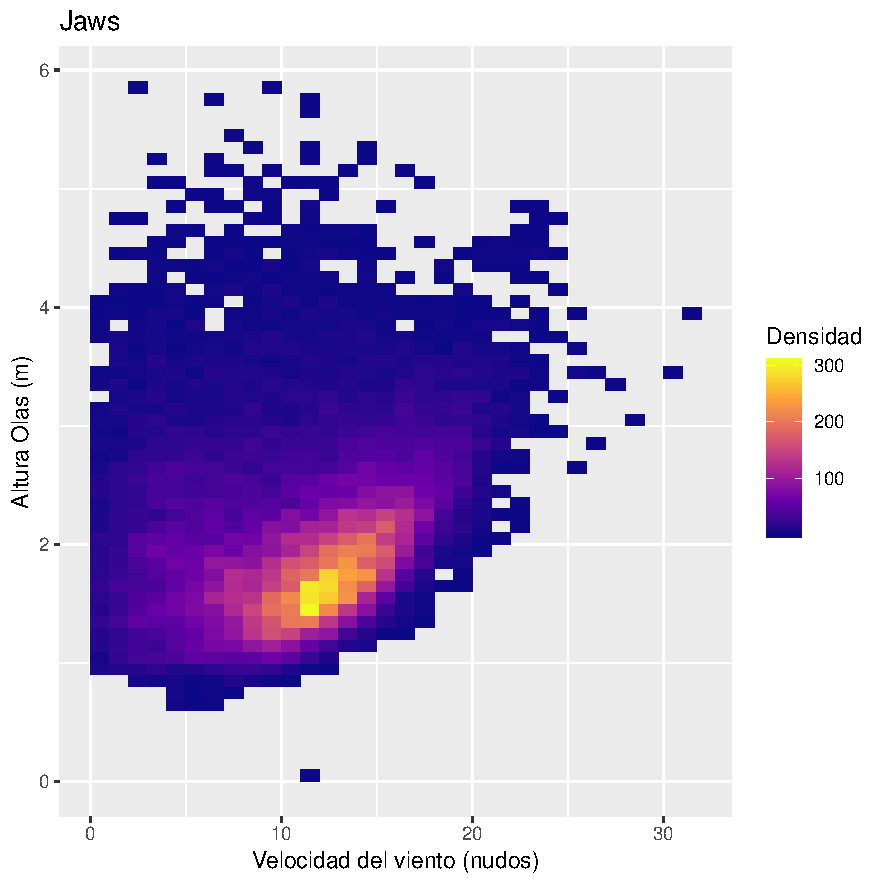
\includegraphics[width=0.6\textwidth]{./figures/jaws.pdf}
  \caption{Velocidad de viento vs. Altura de olas en Jaws en Peahi, Hawái}
\end{figure}

\begin{figure}[!ht]
\label{fig:wind_waves_nazare}
\centering
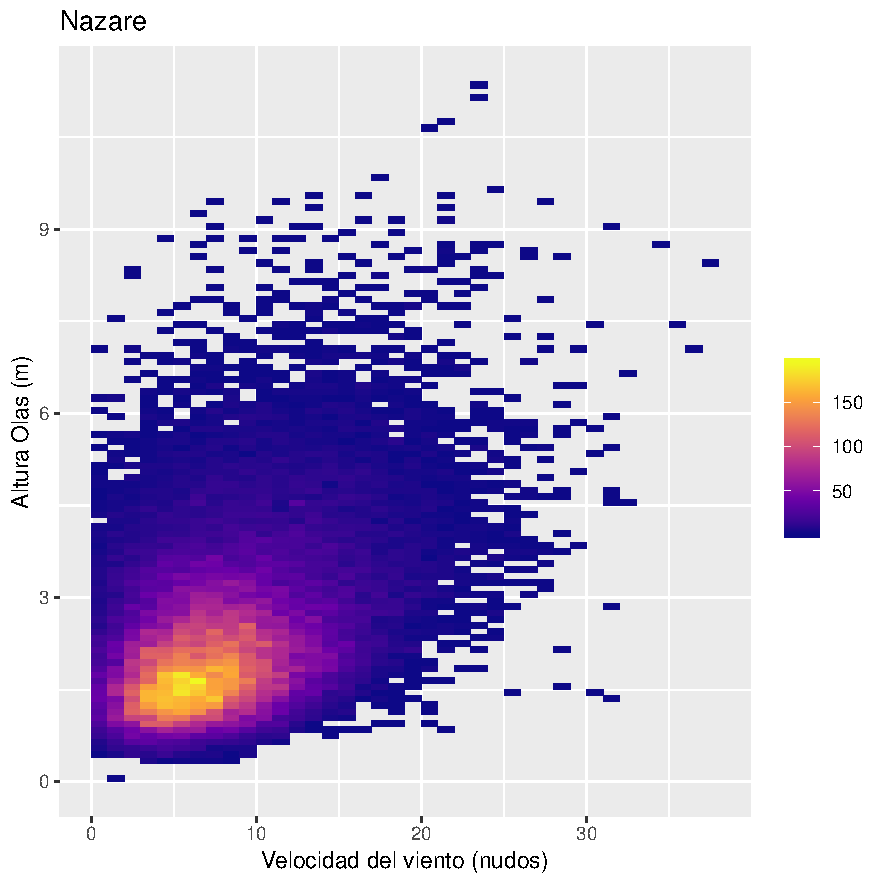
\includegraphics[width=0.6\textwidth]{./figures/nazare.pdf}
  \caption{Velocidad de viento vs. Altura de olas en Nazaré, Portugal}
\end{figure}



\section{Discusión}%
\label{sec:discusión}


\pagebreak
\appendix

\section{Código extracción de datos}%
\label{sec:codigo_extraccion_de_datos}

\lstinputlisting[language=Python]{./process.py}

\end{document}

% vim:sw=2:ts=2:et:spell:spelllang=es:
